%Autor:		Nithuran Selvarajah
%Version:	1.0
%Datum:		21.12.2019

\iffalse
\begin{graphPlot}
	{
		\draw[red, ultra thick, domain=0.01:2] plot (\x, {\x});				% Steigende Gerade
	}
\end{graphPlot}
\fi

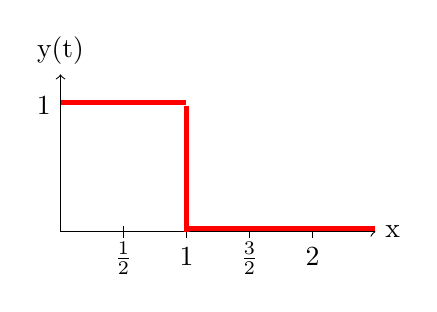
\begin{tikzpicture}[xscale=0.8, yscale=0.8]
	%\draw[help lines] (0,0) grid (6,4);
	\normalsize
	
	\draw [<->] (0, 2.5) -- (0, 0) -- (5, 0);
	\node [right] at (5, 0) {x};				% x-label
	\node [above] at (0, 2.5) {y(t)};			% y-label
	
	\draw (1, -0.1) --  (1, 0.1);				% Strich
	\node [below] at (1, 0) {$\frac{1}{2}$};	% Zahl beim Strich
	\draw (2, -0.1) --  (2, 0.1);
	\node [below] at (2, -0.1) {$1$};
	\draw (3, -0.1) --  (3, 0.1);
	\node [below] at (3, 0) {$\frac{3}{2}$};
	\draw (4, -0.1) --  (4, 0.1);
	\node [below] at (4, -0.1) {$2$};
	
	\node [left] at (0,2) {$1$};
	%\draw [-, red] (0, 3) -- (5, 3);			% Gerade Linie
	\draw[red, ultra thick, domain=0.01:2] plot (\x, {2.05});		% Konstante
	\draw[red, ultra thick] (2, 0) -- (2, 2);						% Senkrechter Strich
	\draw[red, ultra thick, domain=0.01:3] plot (\x + 2, {0.05});	% Konstante

\end{tikzpicture}
